\documentclass{article}

\usepackage[utf8]{inputenc}
\usepackage{amsthm}
\usepackage{amssymb}
\usepackage{mathtools}
\usepackage{graphicx}
\usepackage{mdframed}
\usepackage{float}
\usepackage[top=0.75in, bottom=0.75in, left=0.75in, right=0.75in]{geometry}
\usepackage{gauss}

\usepackage{array}
\allowdisplaybreaks

\makeatletter
\newcounter{elimination@steps}
\newcolumntype{R}[1]{>{\raggedleft\arraybackslash$}p{#1}<{$}}
\def\elimination@num@rights{}
\def\elimination@num@variables{}
\def\elimination@col@width{}
\newenvironment{elimination}[4][0]
{
    \setcounter{elimination@steps}{0}
    \def\elimination@num@rights{#1}
    \def\elimination@num@variables{#2}
    \def\elimination@col@width{#3}
    \renewcommand{\arraystretch}{#4}
    \start@align\@ne\st@rredtrue\m@ne
}
{
    \endalign
    \ignorespacesafterend
}
\newcommand{\step}[2]
{
    \ifnum\value{elimination@steps}>0\sim\quad\fi
    \left[
        \ifnum\elimination@num@rights>0
            \begin{array}
            {@{}*{\elimination@num@variables}{R{\elimination@col@width}}
            |@{}*{\elimination@num@rights}{R{\elimination@col@width}}}
        \else
            \begin{array}
            {@{}*{\elimination@num@variables}{R{\elimination@col@width}}}
        \fi
            #1
        \end{array}
    \right]
    & 
    \begin{array}{l}
        #2
    \end{array}
    \addtocounter{elimination@steps}{1}
}
\makeatother

\DeclarePairedDelimiter{\abs}{\lvert}{\rvert}
\DeclarePairedDelimiter{\norm}{\lvert \lvert}{\rvert \rvert}

\newtheoremstyle{break}% name
  {}%         Space above, empty = `usual value'
  {}%         Space below
  {\itshape}% Body font
  {}%         Indent amount (empty = no indent, \parindent = para indent)
  {\bfseries}% Thm head font
  {.}%        Punctuation after thm head
  {\newline}% Space after thm head: \newline = linebreak
  {}%         Thm head spec

\newtheorem{Def}{Definition}[section]

\theoremstyle{break}

\newtheorem{innerEx}{Exempel}[section]
\newtheorem{sats}{Sats}[section]
\newtheorem{Rem}{Anmärkning}[]

\newenvironment{Ex}
{\begin{mdframed} \begin{innerEx} \vspace{3pt}}
{\vspace{3pt} \end{innerEx} \end{mdframed}}  

\newenvironment{bevis}
{\begin{mdframed} \begin{proof} \vspace{3pt}}
{\vspace{3pt} \end{proof} \end{mdframed}}


\title{
     Analys\\
     Föreläsning 1 - Reella tal och absolutbelopp
    \author{Erik Sjöström}
}
\begin{document}
\maketitle

\section{Reella tal}

\begin{center}
    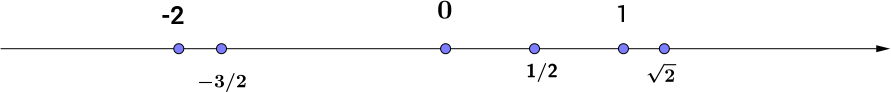
\includegraphics[scale=0.5]{linje.png}
\end{center}

\begin{itemize}
    \item $\mathbb{R}$ = mängden av reella tal\\
    \item $a \in \mathbb{R}$ = a är ett element i $\mathbb{R}$ (a är ett reellt tal)
\end{itemize}

\subsection{Algebraiska egenskaper} % (fold)
\label{sub:algebraiska_egenskaper}

\[
a,b \in \mathbb{R} \Rightarrow a + b, a - b, a \cdot b, \frac{a}{b} \in \mathbb{R} \mbox{ }(a \neq 0, b \neq 0)
\]
% subsection algebraiska_egenskaper (end)

\subsection{Ordningsrelation på $\mathbb{R}$} % (fold)
\label{sub:ordningsrelation_p_}
\begin{itemize}
    \item $a < b$ om:
    \begin{center}
        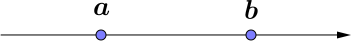
\includegraphics[scale=0.5]{mindre.png}
    \end{center}
    \item $a > b$ om:
    \begin{center}
        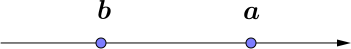
\includegraphics[scale=0.5]{storre.png}
    \end{center}
    \item $a \le b$ om $a < b$ eller $a = b$
\end{itemize}
% subsection ordningsrelation_p_ (end)
\subsection{Räkneregler, $a, b \in \mathbb{R}$} % (fold)
\label{sub:r_kneregler_}
\begin{itemize}
    \item $c \in \mathbb{R}$, $a < b$ $\Rightarrow$ $(a + c) < (b + c)$
    \item $c \in \mathbb{R}$, $c > 0$ , $a < b$ $\Rightarrow$ $(a \cdot c) < (b \cdot c)$
    \item $c \in \mathbb{R}$, $c < 0$, $a < b$ $\Rightarrow$ $(a \cdot c) > (b \cdot c)$
\end{itemize}
\begin{Ex}
    Bestäm $x \in \mathbb{R}$ så att:
    \[
    1 \le 2x + 3 < 5
    \]
    Vi har:
    \begin{align*}
        \{x \in \mathbb{R}: 1 \le 2x + 3 < 5\} &= \{x \in \mathbb{R}: 1 \le 2x + 3, \mbox{ och }, 2x + 3 < 5\} \\
        &= \{x \in \mathbb{R}: -2 \le 2x, \mbox{ och }, 2x < 2\} \\
        &= \{x \in \mathbb{R}: -1 \le x, \mbox{ och }, x < 1\} \\
        &= \{x \in \mathbb{R}: -1 \le x < 1\}
    \end{align*}
    \begin{center}
        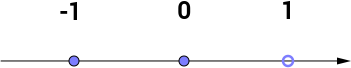
\includegraphics[scale=0.5]{exlinje.png}
    \end{center}
    \[
    = [-1, 1)
    \]
\end{Ex}
% subsection r_kneregler_ (end)
\subsection{Intervallbeteckningar,  $a,b \in \mathbb{R}$, $a \le b$} % (fold)
\label{sub:intervallbeteckningar_}
\begin{itemize}
    \item $(a, b) = \{x \in \mathbb{R}: a < x < b\}$
    \item $[a, b) = \{x \in \mathbb{R}: a \le x < b\}$
    \item $(a, b] = \{x \in \mathbb{R}: a < x \le b\}$
    \item $[a, b] = \{x \in \mathbb{R}: a \le x \le b\}$
\end{itemize}
$-\infty, \infty \notin \mathbb{R}$
\begin{itemize}
    \item $(a, \infty) = \{x \in \mathbb{R}: a < x\}$
    \item $[a, \infty) = \{x \in \mathbb{R}: a \le x\}$
    \item $(-\infty, a) = \{x \in \mathbb{R}: x < a\}$
    \item $(-\infty, a] = \{x \in \mathbb{R}: x \le a\}$
    \item $(-\infty, \infty) = \mathbb{R}$
\end{itemize}

\begin{Ex}
    Bestäm det $x$ som uppfyller olikheten:
    \[
    \frac{x-1}{2} < -5x
    \]
    Lösning:
    \begin{align*}
        \frac{x-1}{2} < -5x &\Leftrightarrow \frac{x-1}{2} + 5x < 0 \\
        &\Leftrightarrow (\frac{1}{2} -5)x - \frac{1}{2} < 0 \\
        &\Leftrightarrow \frac{11}{2}x - \frac{1}{2} < 0 \\
        &\Leftrightarrow \frac{11}{2}x < \frac{1}{2} \\
        &\Leftrightarrow x < \frac{1}{11} \\
        &\Leftrightarrow x \in (-\infty, \frac{1}{11})
    \end{align*}
\end{Ex}
\begin{Ex}
    Bestäm det $x$ som uppfyller olikheten:
    \[
    \frac{x-1}{2} < \frac{-5}{x}
    \]
    Lösning:
    \begin{align*}
        \frac{x-1}{2} < \frac{-5}{x} &\Leftrightarrow \frac{x-1}{2} + \frac{5}{x} < 0 \\
        &\Leftrightarrow \frac{x(x-1) + 5 \cdot 2}{2x} < 0 \\
        &\Leftrightarrow \frac{x^2 - x + 10}{2x} < 0
    \end{align*}
    Kvadratkomplettera!
    \[
    x^2 - x + 10 = (x - \frac{1}{2})^2 - (\frac{1}{2})^2 + 10 = \overbrace{\overbrace{(x - \frac{1}{2})^2}^{\ge 0} + \frac{39}{4}}^\text{= $\frac{39}{4}$ då x = $\frac{1}{2}$} \ge \frac{39}{4} > 0
    \]
    Alltså:
    \[
    \{x \in \mathbb{R}: \frac{x-1}{2} < \frac{-5}{x}\} = \{x \in \mathbb{R}: \frac{x^2 - x + 10}{2x} < 0 \} = \{x \in \mathbb{R}: x < 0\} = (-\infty, 0)
    \]
\end{Ex}
% subsection intervallbeteckningar_ (end)
\section{Absolutbelopp} % (fold)
\label{sec:absolutbelopp}
\begin{Def}
    \[
    \abs{a} =
    \begin{cases}
        a \mbox{ om } \ge 0\\
        -a \mbox{ om } < 0
    \end{cases}
    \]
    dvs $\abs{a}$ = avståndet mellan 0 och a.
\end{Def}
Sätt $f(x) = \abs{x}$:
\begin{center}
    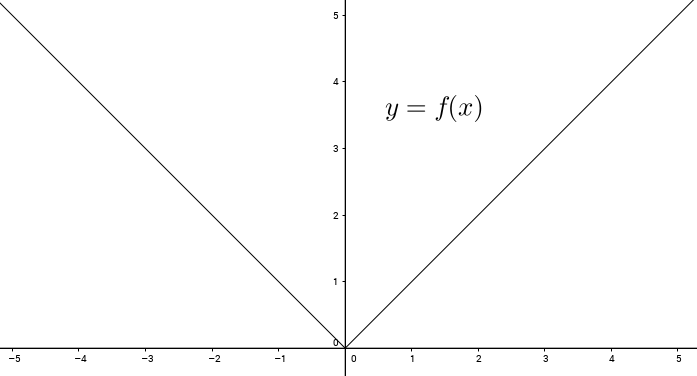
\includegraphics[scale=0.5]{graf.png}
\end{center}
\subsection{Räkneregler $a,b \in \mathbb{R}$} % (fold)
\label{sub:r_kneregler_1}
\begin{itemize}
    \item $\abs{-a} = \abs{a}$
    \item $\abs{ab} = \abs{a} \cdot \abs{b}$
    \item $\abs{a + b} \le \abs{a} + \abs{b}$ (triangelolikheten)
    \item $a \le \abs{a}$
    \item $\abs{a} < b \Leftrightarrow -b < a < b$
\end{itemize}
% subsection r_kneregfeler_ (end)
% section absolutbelopp (end)
\begin{Ex}
    Bestäm $x \in \mathbb{R}$ så att:
    \[
    \abs{x^2 - 5x + 6} < 1
    \]
    \textbf{Metod 1:}
    \[
    -1 < x^2  -5x + 6 < 1
    \]
    \textbf{Metod 2:}
    \begin{center}
        Dela upp i olika fall.
    \end{center}
    \textbf{Metod 3:}
    \begin{center}
        Studera grafen till $f(x) = \abs{x^2 - 5x + 6}$
    \end{center}
\end{Ex}
\end{document}